\chapter{Robotic Foundation Models}
\label{sec:rfms}

The term ``foundation model'' in \ac{AI} refers to large models (often trained on vast data from the internet) that provide a general base which can be adapted to many downstream tasks. In robotics, foundation models are emerging as a way to achieve generalist behavior across many tasks and environments, leveraging multimodal understanding. Two lines of work converged here: (a) multi-task learning in robotics, where a single network is trained to perform many different tasks (across possibly different embodiments), and (b) vision-language models that exhibit general-purpose understanding and reasoning. The combination leads to \ac{VLA} models; policies that ingest visual observations and language instructions, and output robotic actions.

\section{Transformer Foundation Models}

The early work on Gato demonstrated transformer-based generalism across multiple domains. Gato was trained on 604 distinct tasks spanning vision, language, and control, from captioning images to playing Atari games and controlling a real robot arm \cite{GATO2022}. With a single set of weights, Gato could accomplish diverse tasks, including robotic manipulations. For instance, on a real-robot block stacking benchmark, Gato could stack objects of novel shapes with success rates comparable to a specialized imitation-learning policy \cite{GATO2022}. This suggests that large transformers can learn a multi-task prior that generalizes to some new variations. However, Gato’s performance also underscored limitations: while it mastered many training tasks, solving an entirely new task outside its training distribution still required fine-tuning or additional data \cite{GATO2022}.

Transformers have also been applied to narrow domains such as planning. SayCan used an \ac{LLM} to interpret high-level instructions and suggest possible robot actions, which were then executed by low-level policies \cite{SAYCAN2022}. SayCan demonstrated robots responding to commands like ``bring me a water bottle'' by decomposing them, but the approach was modular (LLM + separate learned skills) rather than end-to-end.

PaLM-E (Embodied PaLM) is another broad model, embedding sensor observations into a language model context, enabling a form of \ac{LLM}-planning for robotics (e.g. reasoning about visual inputs and issuing actions) \cite{PALM2023}. These broader models extend the concept of a ``robotic foundation model'' beyond just direct visuomotor policies, towards multimodal reasoning agents. The theoretical promise is an embodied general intelligence that flexibly applies knowledge to new scenarios, yet practically they reveal how far current models must go to truly generalize in the real world.

A landmark was Robotics Transformer 1 (RT-1), which collected 130,000 demonstrations across 700+ household tasks for a mobile manipulator and trained a Transformer policy that takes image and textual goal description, and outputs motor commands \cite{RT12022}. RT-1 achieved robust multi-task performance (e.g. picking up arbitrary objects specified by language) within its training distribution. 

\section{VLA Foundation Models}

\subsection{Architecture}

Recent breakthroughs introduce \ac{VLA} models as large-scale ``foundation'' policies that integrate vision and language understanding to directly generate low-level robot actions. By leveraging pre-trained vision-language knowledge from the web and massive multi-task training, these models aim to provide generalist skills out-of-the-box and zero-shot adaptation to new instructions, drastically reducing the need for task-specific programming or extensive new demonstrations.

\acp{VLA} extend the capabilities of \acp{VLM} and \acp{LLM} by incorporating an action-generation component, as illustrated in \cref{fig:vla-arch}. These models unify perception and instruction understanding into an end-to-end system that produces control outputs, enabling robots to act on internet-scale knowledge with minimal task-specific engineering.

\begin{figure}[ht]
    \centering
    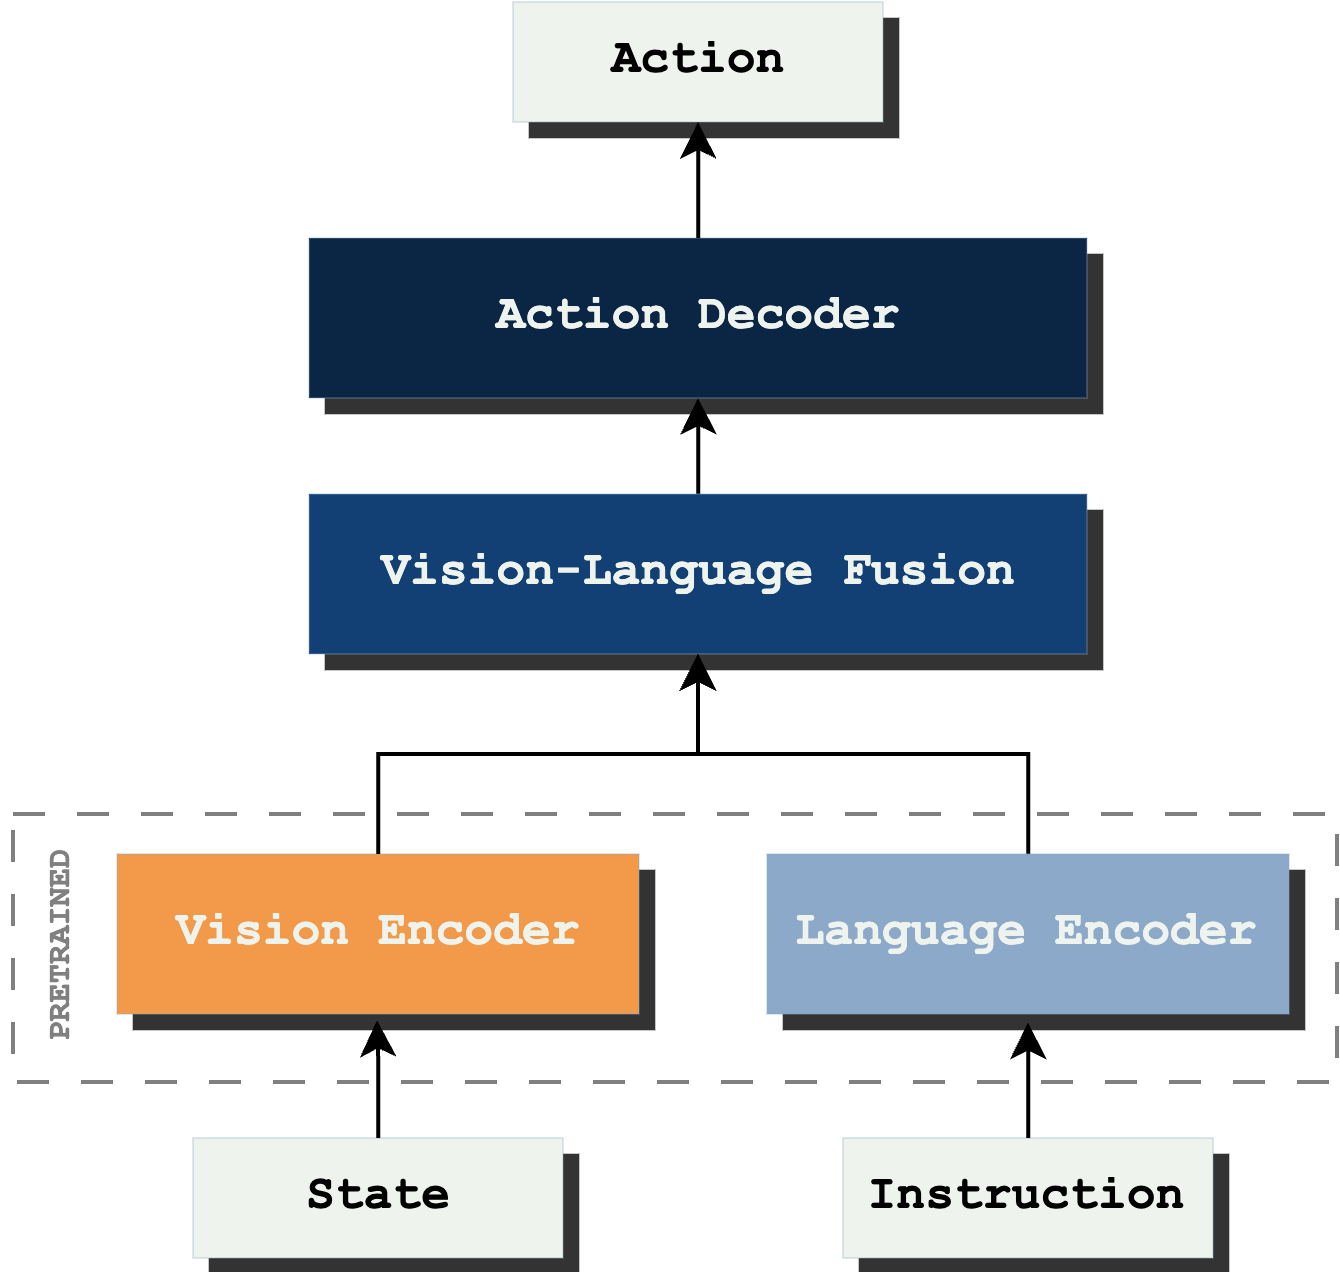
\includegraphics[width=0.5\textwidth]{Figures/vla-arch.png}
    \caption{\ac{VLA} architecture. A pretrained vision encoder ingests the robot's state and a pretrained language encoder processes the instruction. Their outputs feed into a shared action decoder, which generates the final action command.}
    \label{fig:vla-arch}
\end{figure}

The current landscape of \ac{VLA} models employ a variety of visual encoder backbones, namely \acp{CNN} \cite{MCIL2021,HULC2022,HULC++2022,PERACT2023, MTACT2024,OCTO2024}, ResNets \cite{CLIPORT2022,ACT3D2023,RVT2023,RVT22024,BCZ2022,ACT2023,DIFFPOLICY2023,SUDD2023, INTLANG2023, GATO2022}, EfficientNets \cite{QTRANSFORMER2023,RTTRAJ2023, RT12022}, \acp{ViT} \cite{LANGCOSTS2022,ROBOPOINT2024,VIMA2023,FLAMINGO2024,VOXPOSER2023,RTH2024,RTX2024, PI02024, OPENVLA2024, GR00T2025}, and hybrid \ac{ViT}-ResNets \cite{MDT2024} to compress visual input into a feature $v \in \mathbb R^{d_v}$. Each leverages different inductive biases, offering a spectrum of trade-offs between representational richness and computational efficiency \cite{VLASURVEY2025}. \acp{ViT} have exhibited superior accuracy relative to \ac{CNN} architectures under data-rich regimes, while requiring substantially less compute to train \cite{16x162021}. 

Visual encoding is only one half of the encoding process. Language encoders often use either a \ac{GPT} decoder-only \cite{CLIPORT2022, LANGCOSTS2022, INTLANG2023, PERACT2023, ACT3D2023, RVT2023, RVT22024, ROBOPOINT2024, FLAMINGO2024, VOXPOSER2023, SUDD2023, MDT2024}, \ac{BERT} encoder-only \cite{HULC2022, HULC++2022} or encoder-decoder \cite{BCZ2022, RT12022, QTRANSFORMER2023, VIMA2023, OCTO2024, RT22023, RTH2024, RTX2024} architecture to compress language input into a feature $\ell \in \mathbb R^{d_{\ell}}$. Relative performance of \ac{GPT} and \ac{BERT}-style models varies across different tasks e.g., paraphrasing vs predicting \cite{BERTGPT2023}.

The vision language fusion module then computes a joint representation $f = \psi(v, \ell) \in \mathbb R^{d_f}$ via cross-attention or \ac{FiLM} \cite{FiLM2017} for an action-decoder to produce a distribution over actions by 
\begin{equation*}
    \pi(a|f) = \text{softmax}\left(Wf+b\right),
\end{equation*}
where $\mathcal{A} = \{a_1, a_2, \ldots, a_{n}\}$, $W\in \mathbb R^{|\mathcal{A}|\times d_f}$ and $b \in \mathbb{R}^{|\mathcal{A}|}$. The final action output might include 6-\ac{DoF} \ac{SE3} end-effector velocities $a = [\dot{x}, \dot{y}, \dot{z}, \dot{\phi}, \dot{\theta}, \dot{\psi}]$, a binary gripper command \cite{RT22023} and the mean and covariance of the uncertainty in the velocities $a\sim \mathcal{N}(\mu_f, \Sigma_f)$ \cite{FLAMINGO2024, VOXPOSER2023}.

\subsection{Comparative Analysis}

Building on the architectural overview above, we now compare five representative \ac{VLA} systems across shared design axes and real-world benchmarks. RT-2 integrates a \ac{ViT} visual encoder with a \ac{GPT}-style decoder and softmax action head, yielding 62\% zero-shot success on novel-object pick-and-place tasks, an improvement from its predecessor RT-1 \cite{RT12022} driven by web-scale vision pretraining \cite{RT22023}. Gemini-ER combines a \ac{ViT} backbone and encoder–decoder language model, achieving a two-fold gain on generalization benchmarks by leveraging dual-stage fine-tuning across Internet and robot data \cite{GEMER2025}. NVIDIA's GR00T N1 emphasizes data efficiency: minimal on-robot tuning on a bimanual humanoid platform delivers 76.8\% average success, reflecting its lightweight ResNet-\ac{FiLM} fusion \cite{GR00T2025}. Figure AI’s Helix adopts separate slow (7 Hz) reasoning and fast (200 Hz) visuomotor loops, enabling high-frequency control of thousands of novel objects and robots \cite{HELIX2025}. Physical Intelligence’s $\pi_0$ model added a flow-matching policy head atop a pre-trained vision-language backbone, training on the largest cross-embodiment dataset to date and generating high-frequency continuous trajectories for 68 tasks over eight robotic platforms \cite{PI02024}. Its successor, $\pi_{0.5}$, incorporated 400 hours of teleoperated data from 100 environments and multiple embodiments, demonstrating superior real-world generalization by contraining on heterogeneous dataset \cite{PI0.52025}. While these results showcase the power of diverse encoder–fusion–head pipelines, direct comparisons as shown in \cref{tab:vla_eval} remain challenging due to inconsistent benchmarks and reporting. Standardized ablations of fusion strategies and unified evaluation suites are needed to identify which architectural choices most strongly drive data efficiency, generalization and control precision.

\Cref{fig:vla-taxonomy} highlights control frequency as a critical axis for real-time, continuous motor control. Models with large vision-language backbones such as PaLM-E and Gemini-ER often struggle to sustain fast inference rates and require special hardware to run, limiting their applicability in tasks requiring sub-millisecond feedback in embedded systems \cite{GEMER2025}. A dual-system design mitigates this bottleneck by decoupling high-level reasoning from low-level control: a lightweight, high-frequency (100–500 Hz) policy handles continuous actions, while the \ac{VLM} operates at slower rates to manage complex perception and planning. This separation underpins the modularity axis, allowing each subsystem to be optimized for its specific temporal demands and ensuring both rapid response and sophisticated interpretation.

% TODO
% \begin{importantbox}
% Despite only focusing on a few VLAs \cite{PI02024, HELIX2025, GEMER2025, GR00T2025, RT22023, OPENVLA2024, OCTO2024} they still do stand on the shoulders of multiple years of progress in both language modeling and multimodality \cite{MCIL2021,HULC2022,HULC++2022,PERACT2023, MTACT2024,OCTO2024, CLIPORT2022,ACT3D2023,RVT2023,RVT22024,BCZ2022,ACT2023,DIFFPOLICY2023,SUDD2023, INTLANG2023, GATO2022, QTRANSFORMER2023,RTTRAJ2023, RT12022, LANGCOSTS2022,ROBOPOINT2024,VIMA2023,FLAMINGO2024,VOXPOSER2023,RTH2024,RTX2024, PI02024, OPENVLA2024, GR00T2025}.
% \end{importantbox}

\begin{figure}[ht]
    \centering
    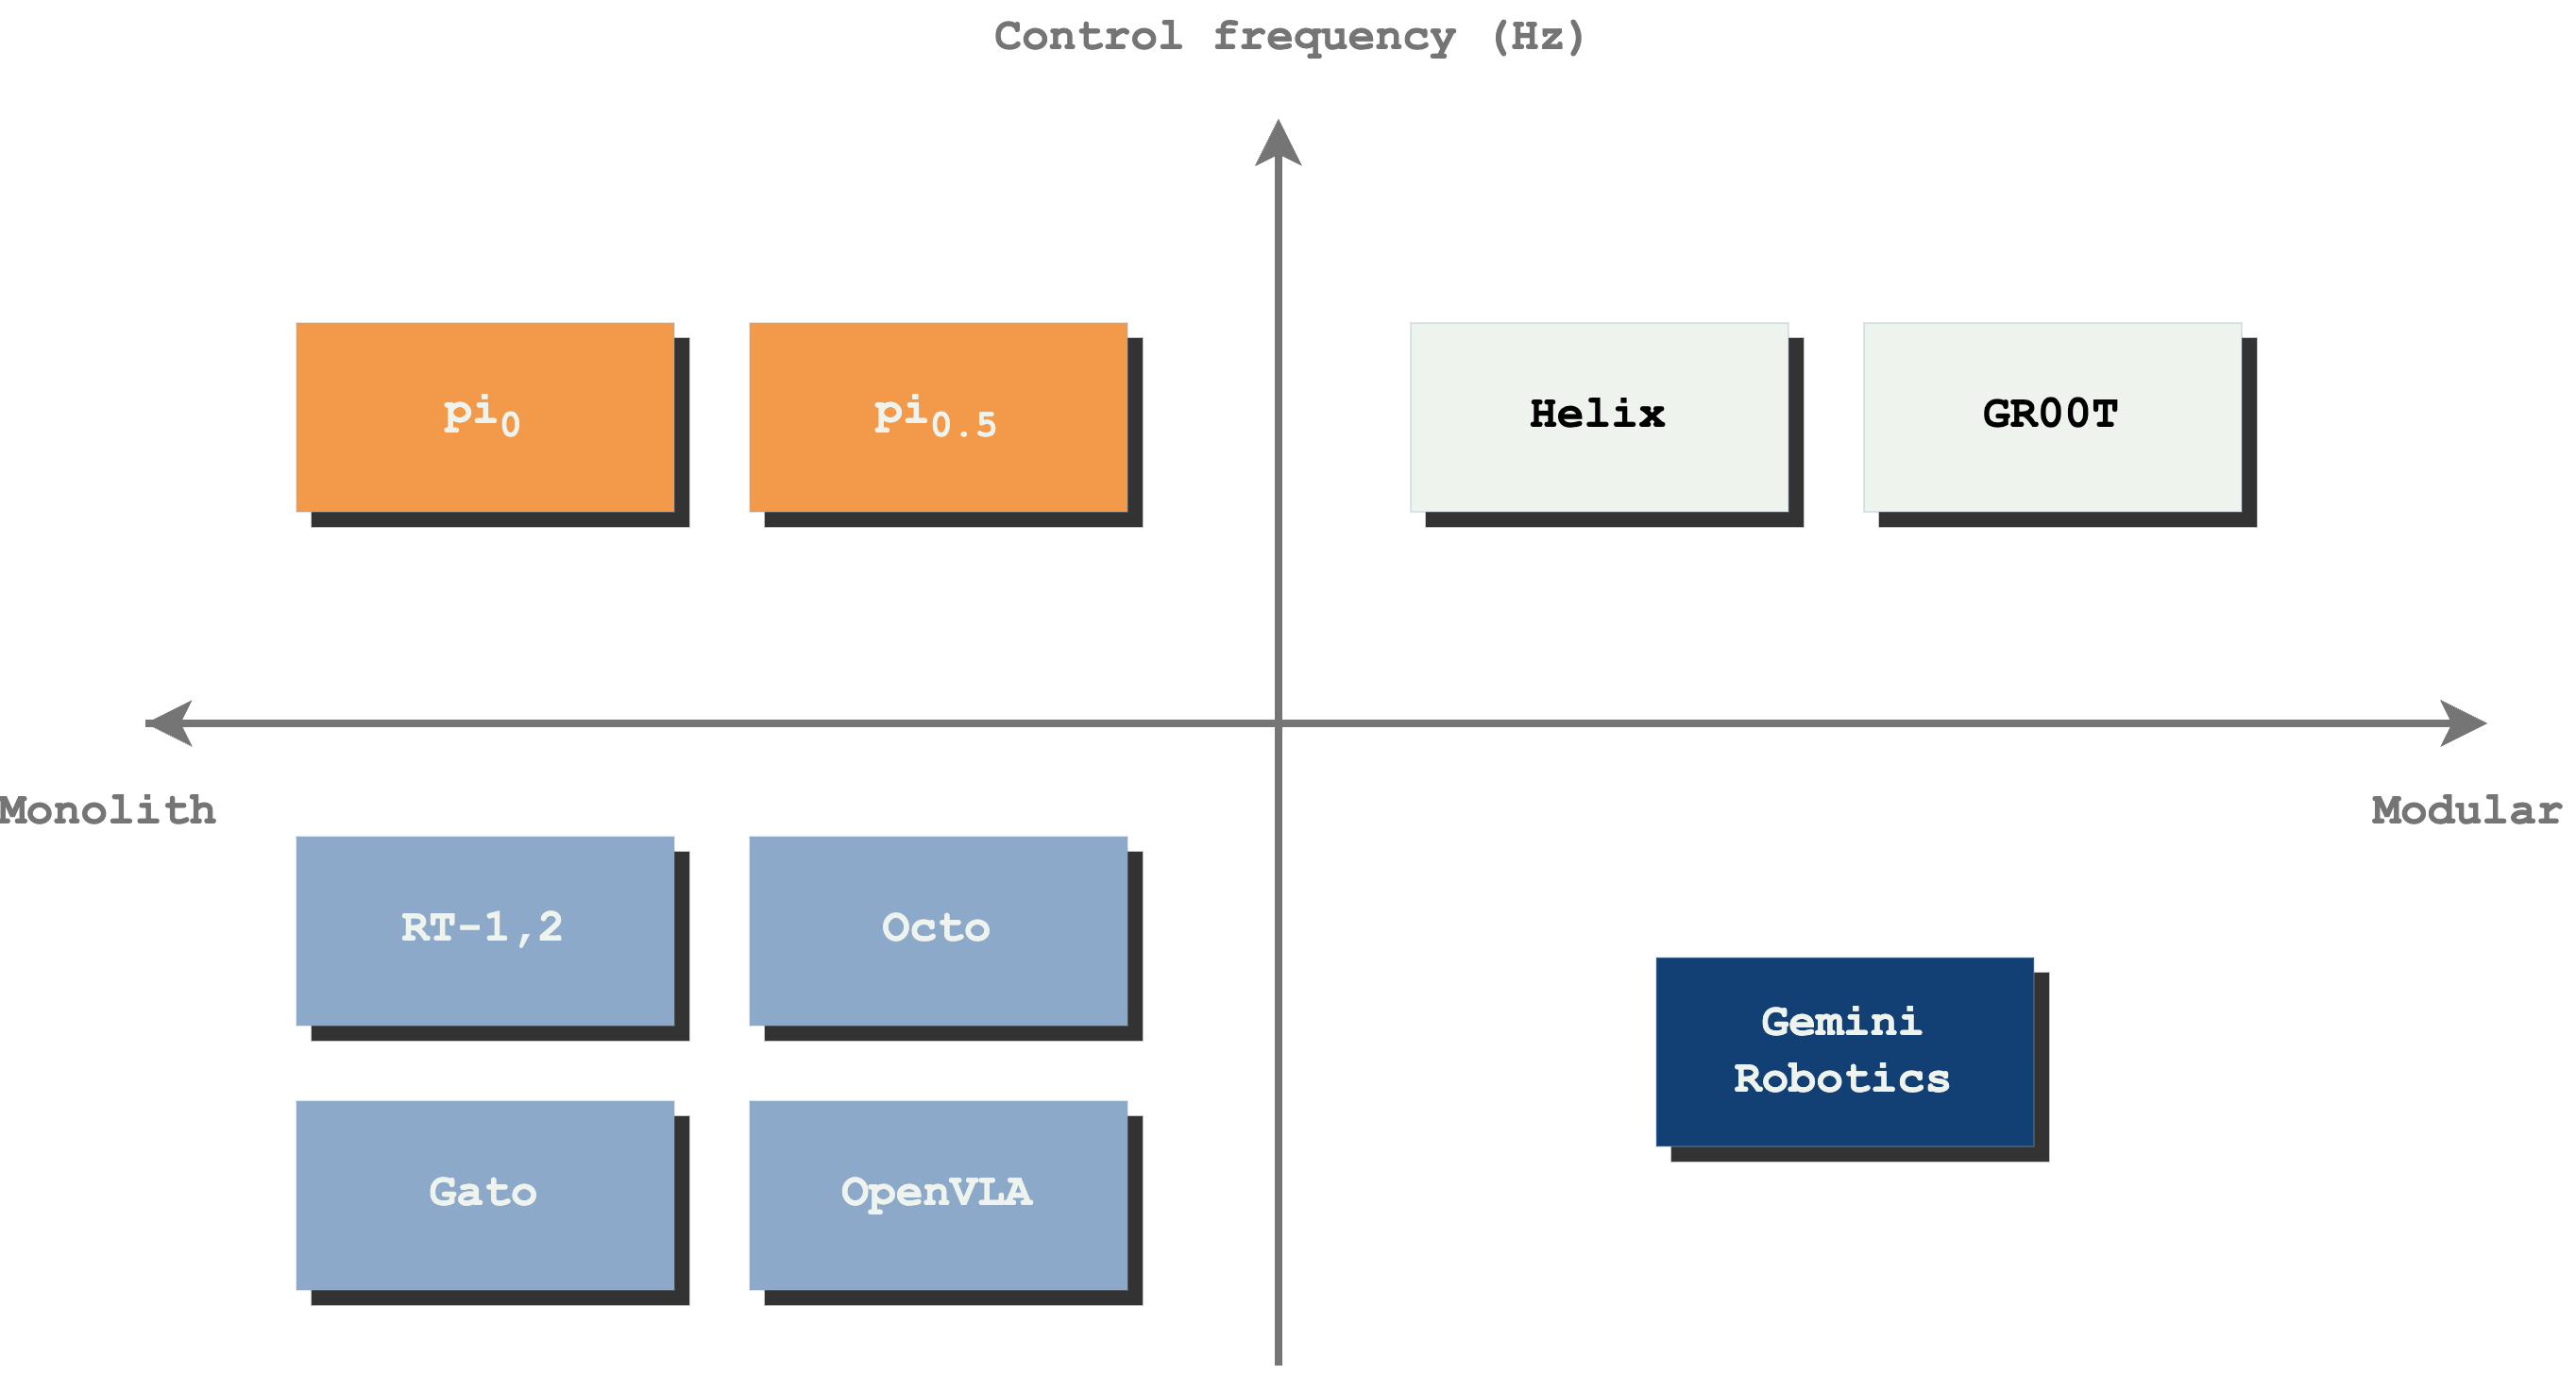
\includegraphics[width=1.0\textwidth]{Figures/taxonomy.png}
    \caption{Taxonomy of Robotic Foundation Models along the axes of Modularity (horizontal) and Control Frequency (vertical). Models in the upper half exhibit higher embodiment coupling (e.g., proprioceptive inputs, closed-loop control), while those on the right are more modular, decoupling perception, reasoning, and control.}
    \label{fig:vla-taxonomy}
\end{figure}

% TODO
% \begin{importantbox}
% Missing paragraph that ties \cref{fig:vla-taxonomy} into \cref{tab:vla_eval}...

% ... the results above show the increase in VLA realibility however they will follow a similar trajectory LLMs have... there isn't enough data to make them smart enough to be general enough to do anything a human can... this is why we need new techniques. Plug to RL.
% \end{importantbox}

\begin{widetable}[htbp]
  \footnotesize
  \begin{threeparttable}
    \caption[Real-world task success rates for VLA models]{Real-world task success rates for \ac{VLA} models. These average success rates were measured under diverse evaluation protocols and do not capture important nuances in real-world benchmarking. Differences in task definitions, completion criteria, environment variability, sensor noise, hardware configurations and quality-assurance procedures mean that values are not strictly comparable across models. Readers should interpret these rates in the context of each model's specific testing methodology.}
    \label{tab:vla_eval}

    \begin{tabularx}{\linewidth}{@{}>{\RaggedRight\arraybackslash}X l l r @{}}
      \toprule
      \tableheadline{Model} &
      \tableheadline{Avg.\ success rate (\%)} &
      \tableheadline{Model size} &
      \tableheadline{Training (steps)} \\
      \midrule
      Gato \cite{GATO2022}         & 50.0\tnote{a} & 1.18B             & 1M          \\
      RT-1 \cite{RT12022}          & 97.0\tnote{b} & 35.0M             & 130K        \\
      Octo \cite{OCTO2024}         & 72.0\tnote{c} & 93.0M             & --          \\
      RT-2 \cite{RT22023}          & 62.0\tnote{d} & 55.0B\tnote{i}    & 80K\tnote{i} \\
      Gemini Robotics \cite{GEMER2025} & 65.0\tnote{e} & --\tnote{*}   & --          \\
      OpenVLA \cite{OPENVLA2024}   & 70.6          & 7.00B             & 970K        \\
      GR00T N1 \cite{GR00T2025}    & 76.8\tnote{f} & 2.00B             & --          \\
      $\pi_{0}$ \cite{PI02024}     & 78.0\tnote{g} & 3.30B\tnote{k}    & 993M\tnote{l} \\
      $\pi_{0.5}$ \cite{PI0.52025} & 82.5\tnote{h} & 3.30B             & 993M+       \\
      \bottomrule
    \end{tabularx}

    \begin{tablenotes}[para,flushleft]
      \footnotesize
      \item[*] Not disclosed but rumored to be 1T+ parameters.\\
      \item[a] $\sim$50\% success on block-stacking of novel objects (5 held-out shapes, 200 trials each) after fine-tuning; on par with single-task expert.\\
      \item[b] $\sim$97\% on seen training tasks (700+ instructions) and $\sim$76\% zero-shot generalization to unseen instructions; tested on Everyday Robots fleet with distractors and novel backgrounds.\\
      \item[c] $\sim$72\% average across six manipulation scenarios (e.g. cable insertion, coffee making, bimanual tasks) after few-shot fine-tuning; $\sim$29\% higher than RT-1-X zero-shot and matched RT-2-X on shared tasks.\\
      \item[d] Measured on novel and unseen tasks using real-robot deployments.\\
      \item[e] Multi-task average across pick-and-place and industrial assembly on a bimanual humanoid platform.\\
      \item[f] Evaluated with few-shot demos on folding, handling, wiping.\\
      \item[g] Consolidated average across pre-training demos for stacking bowls, laundry, bussing and dryer unloading.\\
      \item[h] Similar to (g) but for dishes in sink, items in drawer, laundry and making bed.\\
      \item[i] 55B PaLI-X variant trained over 80K steps and 12B PaLM-E variant over 1M steps.\\
      \item[k] 3.3B = 3.0B \ac{VLM} + 300M action.\\
      \item[l] 993M = 903M from robot demos plus 90M steps from open datasets and task-specific fine-tuning of 1--10h per task.\\
    \end{tablenotes}

  \end{threeparttable}
\end{widetable}


\subsection{Real-World Benchmarks}

To measure progress towards general-purpose, real-world-capable robots, we require benchmarks that test both the breadth and adaptability of robotic intelligence. This section surveys existing benchmarks and proposes criteria for evaluating integrated \ac{RL}-\ac{VLA} systems, with emphasis on real-world performance.

\paragraph{Multi-Task and Generalization Benchmarks.}

Early benchmarks for generalist robots have emerged in simulation. Meta-World is a suite of 50 manipulation tasks (e.g., push button, open door) used to evaluate multi-task learning and meta-learning algorithms. A single policy’s ability to master all Meta-World tasks (and generalize to new ones) is an indicator of general-purpose skill. Another is RLBench, a library of 100+ simulated tasks with diverse tool use and settings, which provides a playground for language-conditioned policies and task generalization. Results from models like $\pi_0$ and Gato on these benchmarks show decent \textit{in-distribution} performance and some ability to adapt to withheld tasks \cite{GATO2022, PI02024}. For example, Gato was evaluated on DM Control Suite tasks and Atari games alongside robotic control, and scaling laws were studied to see performance trends across domains \cite{GATO2022}. However, simulation benchmarks, while useful, often don’t capture the noise and variability of the real world.

\paragraph{Real-World Performance Benchmarks.}

A few benchmarks explicitly target real robot generalization. One notable example is the RGB-Stacking Benchmark introduced by \textcite{PICKPL2021}, where a robot arm must learn to stack novel shapes of blocks by training on some shapes and testing on unseen ones. Gato’s evaluation on RGB-Stacking’s Skill Generalization task showed it could match a specialist policy’s success rate around $\sim$50\% \cite{GATO2022}, providing a quantitative measure of cross-generalization. There are also household task benchmarks, for instance, the BEHAVIOR benchmark (Benchmark for Everyday Household Activities in Virtual, 2021) defines 100 activities (like cleaning a table, making coffee) in simulation but with an eye towards real-world complexity; it has a concept of generalization to new object instances and environments \cite{BEHAV2021}. Some researchers have attempted these tasks on real robots like the Toyota HSR or Stretch, evaluating success in real home settings. Another emerging evaluation is open-vocabulary object manipulation: tests where a robot is asked to pick or arrange objects specified by category or attribute (possibly unseen during training). RT-2 and Helix were implicitly tested on this e.g., ``pick up the strawberry toy'' vs ``pick up the dinosaur toy'' where the latter might be novel. Embodiment transfer could also be considered a benchmark: how well a policy trained on one robot does on another with minimal adjustment (Gemini’s embodiment adaptation is a case study). A crucial piece for real-world benchmarking is measuring robustness and safety: for example, the ``Real-World RL'' suite \cite{CHRL2019} proposes metrics like how often policies fail catastrophically, how much human intervention is needed, etc. For integrated \ac{RL}+\ac{VLA}, we might want a benchmark that requires an agent to understand an instruction, then learn a new skill to fulfil it. Imagine a test where a robot is told, ``Here is a new tool, figure out how to use it to hang this picture,'' success would require comprehension (\ac{VLA}) and on-the-spot learning (\ac{RL}). While no standard benchmark yet captures this full spectrum, individual components exist that can be combined.

\paragraph{Evaluation Criteria and Research Gaps in Benchmarking.}

Current benchmarks often address either generalization \textit{or} learning, but integrated systems need both. Evaluation criteria should include: (a) Generalization to novel objects/tasks (test on things not in training data), (b) Sample efficiency/Adaptation (measure how many trials or demos needed to learn a new task to a certain performance level), (c) Multi-modality (the agent must handle vision, language and possibly other sensors), and (d) Long-horizon performance (tasks requiring many steps, where planning or subgoals are needed). A combination of simulated and real benchmarks is ideal; simulation for rapid testing and ablation, and real for ultimate validation. One gap is the lack of a widely-adopted real-world benchmark suite for generalist robots. This is partly because deploying identical evaluations on physical robots is hard (equipment differences, etc.). Some initiatives, like the REAL Competition \cite{REAL2022} or Roboturk/Robomimic datasets \cite{TURK2016}, push toward standardizing evaluation by providing common environments or datasets. Benchmarking \ac{RL}-\ac{VLA} integration might involve tasks like: follow a novel instruction that requires learning a new behavior (e.g., ``Learn to use this screwdriver to tighten a bolt'' where ``using a screwdriver'' was not in training). Success would be measured by the agent’s ability to figure it out within a limited number of tries. As research progresses, the community may define challenge tasks akin to a Robotic IQ test that spans reasoning, memory, and learning. For now, researchers rely on assembling evidence across multiple benchmarks: if a new model beats baselines on Meta-World, RGB-Stacking, and perhaps a real kitchen task, this is considered progress. In conclusion, developing better benchmarks is itself an open problem, necessary to drive the field toward truly general-purpose robotic intelligence.

\section[Generalization in Real-World Environments]{Generalization in Real-World Environments: Current State and Gaps}

While foundation models show impressive generalist capabilities in lab settings, their ability to handle the open-ended complexity of the real world is limited. This section examines the state-of-the-art in real-world capable transformer-based robotic learning and identifies gaps in generalization and online learning.

\paragraph{Robustness and Distribution Shift.}

Transformer-based policies often face a reality gap when moving from curated training data to unstructured real environments. Even the best \ac{VLA} models can struggle with \ac{OOD} scenarios i.e., situations not seen during training. For instance, a model trained on indoor tabletop manipulation might falter in a completely new setting (say, outdoors or in a cluttered home with novel object types). Generalization is typically tested by holding out some object types or task variations. As noted, Gato’s real-robot evaluation involved stacking objects of unseen shapes, where it achieved moderate success \cite{GATO2022}.

Similarly, RT-2 was demonstrated to handle some novel objects and instructions beyond its direct robot experience. However, these cases remain relatively constrained (novel combinations of familiar elements) \cite{RT22023}. Truly entirely unseen environments, with new lighting conditions, unfamiliar object categories, or unforeseen physics remain a tough challenge. The current state is that no transformer-based robotic agent can yet be deployed to any arbitrary real-world environment with reliable performance. Safety and reliability concerns also emerge: models might misinterpret unusual inputs, leading to unsafe actions. A research gap here is how to make these large models more robust to distribution shift, possibly through better simulation-to-real transfer, domain randomization, or online adaptation.

\paragraph{Lack of Online Learning and Adaptation.}

Most transformer-based policies are trained offline and then frozen (or only lightly fine-tuned) before deployment. In contrast, human and animal intelligence continuously learns from experience in real time. Current systems have little ability to improve on the fly when faced with new challenges. For example, if a robot encounters a tool it has never seen, a fixed model can only rely on its prior knowledge (which might be insufficient), whereas an ideal agent would experiment and learn about the tool. Online \ac{RL} (or other forms of continual learning) are generally absent from \ac{VLA} pipelines. This is a significant gap: without online learning, models cannot systematically improve in new environments or recover from errors by refining their policy. Some initial efforts are exploring this e.g., using \ac{RL} fine-tuning to improve pretrained \ac{VLA} models \cite{IREVLA2025} but integrating real-time learning remains an open research area. Challenges include catastrophic forgetting (learning new things without overwriting old knowledge) and safety during exploration. Thus, a crucial research direction is how to imbue transformer-based agents with online adaptation, possibly through hybrid architectures or constrained exploration that keeps the robot and its environment safe.

\paragraph{Sample Efficiency and Real-World Data Constraints.}

In real-world robotics, collecting data is expensive and time-consuming, which makes sample efficiency pivotal. Yet many transformer-based approaches demand huge datasets. \ac{VLA} models like RT-2, Gemini-ER and $\pi_o$ are enabled by internet-scale pretraining or thousands of human demonstrations \cite{RT22023, GEMER2025, PI02024}. This raises concerns: can these models generalize without such extensive data for every new situation? Current evidence suggests diminishing returns when encountering scenarios not covered by training data. For instance, Gemini Robotics needed additional fine-tuning to specialize in long-horizon tasks or new embodiments, implying that pretraining alone was insufficient for those capabilities. Moreover, models may not generalize to new embodiments (robot hardware) without retraining because the dynamics and kinematics differ. While Gemini reports some success in adapting to new robots via fine-tuning \cite{GEMER2025}, true embodiment-agnostic control remains unsolved. In summary, the current state-of-the-art transformer models mark substantial progress toward real-world robotics, but fall short in generalizing to truly novel situations, learning continuously, and minimizing data requirements. The following sections delve into specific limitations and complementary approaches addressing these issues.

\paragraph{Low-Latency Control.}

Dynamic environments demand not only robust policies but also rapid inference to close the perception-action loop. For smooth locomotion and manipulation, end-to-end latency (from sensor capture to motor command) must often fall within 2–10 ms or 100–500 Hz using $f = 1/T$, to match human-like responsiveness \cite{LOCOSURVEY2025}. Higher latencies introduce perceptible lag, degrading control stability and reducing the agent’s ability to react to unforeseen perturbations. Without real-time inference, even a well-trained model cannot generalize effectively in fast-changing settings; objects move, lighting shifts, and contacts occur unpredictably. Thus, designing transformer-based architectures or deployment pipelines that guarantee low-latency execution (via model compression, distillation, or hardware-aware optimizations) is essential for dependable real-world performance.
